
\begin{figure}[H]
\minipage{0.49\textwidth}
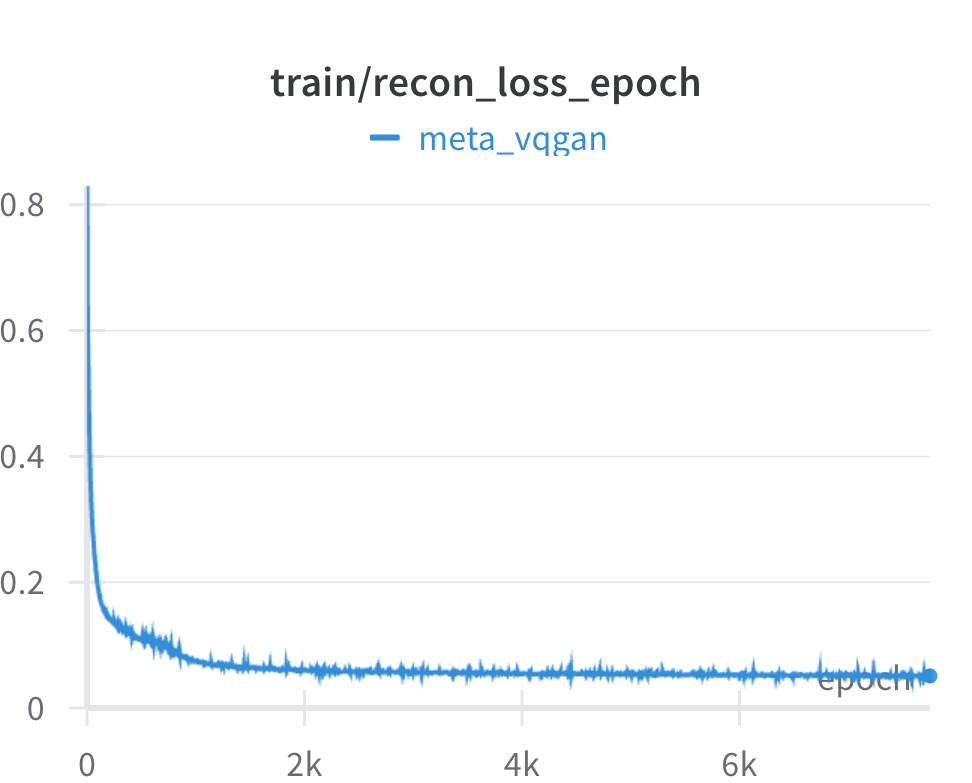
\includegraphics[width=\linewidth]{detailed_engineering/Meta VQGAN/charts/Section-2-Panel-13-1qhe42yar.png}
\caption{Reconstruction loss during the training.}
\endminipage\hfill
\minipage{0.49\textwidth}
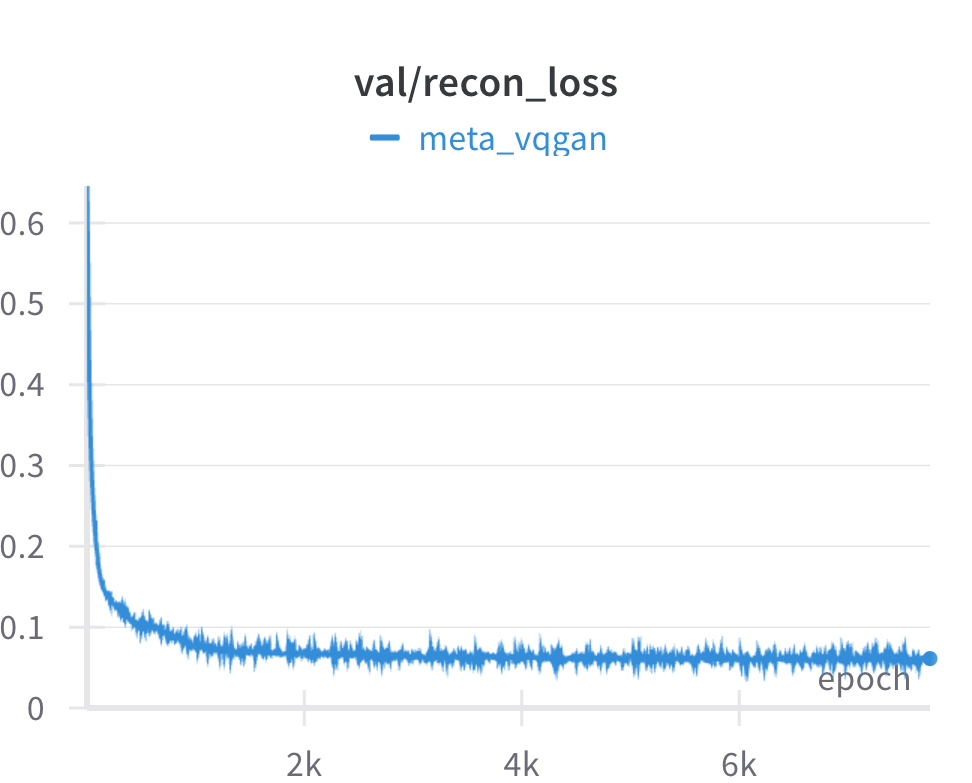
\includegraphics[width=\linewidth]{detailed_engineering/Meta VQGAN/charts/Section-4-Panel-3-hkj1c12xb.png}
\caption{Reconstruction loss during the validation.}
\endminipage
\caption{Reconstruction loss during the training and the validation. Lower is better.}
\end{figure}

\begin{figure}[H]
\minipage{0.49\textwidth}
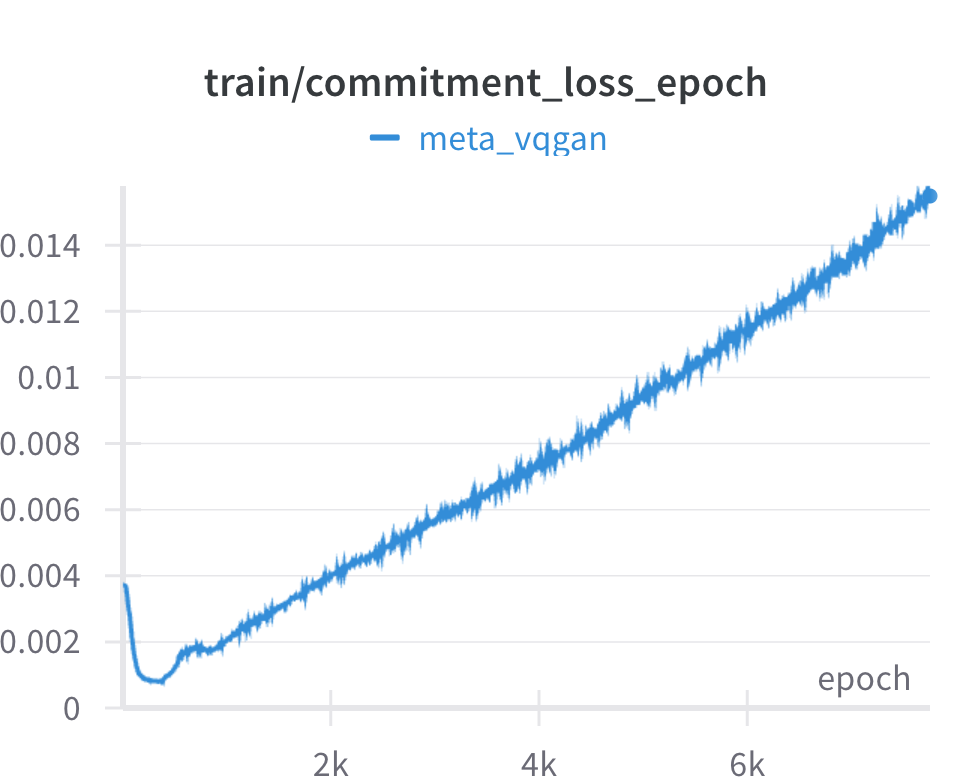
\includegraphics[width=\linewidth]{detailed_engineering/Meta VQGAN/charts/Section-2-Panel-11-4ox8mpc2c.png}
\caption{Perceptual loss during the training.}
\endminipage\hfill
\minipage{0.49\textwidth}
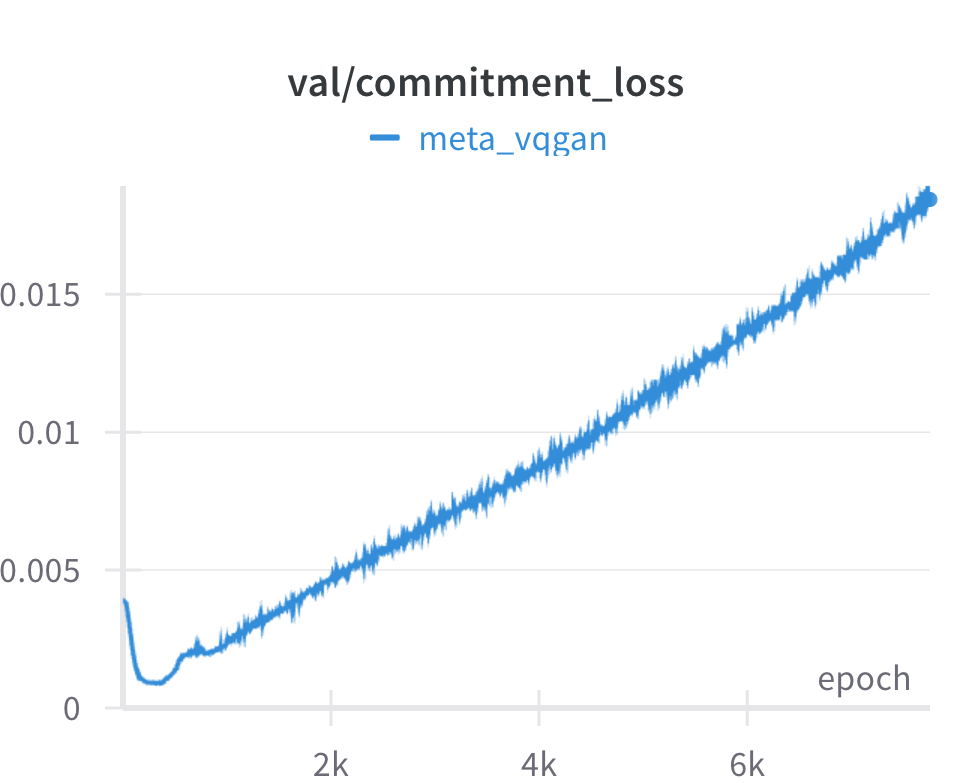
\includegraphics[width=\linewidth]{detailed_engineering/Meta VQGAN/charts/Section-4-Panel-2-2k8ixubhi.png}
\caption{Perceptual loss during the validation.}
\endminipage
\caption{Perceptual loss during the training and the validation. Lower is better.}
\end{figure}

\begin{figure}[H]
\minipage{0.49\textwidth}
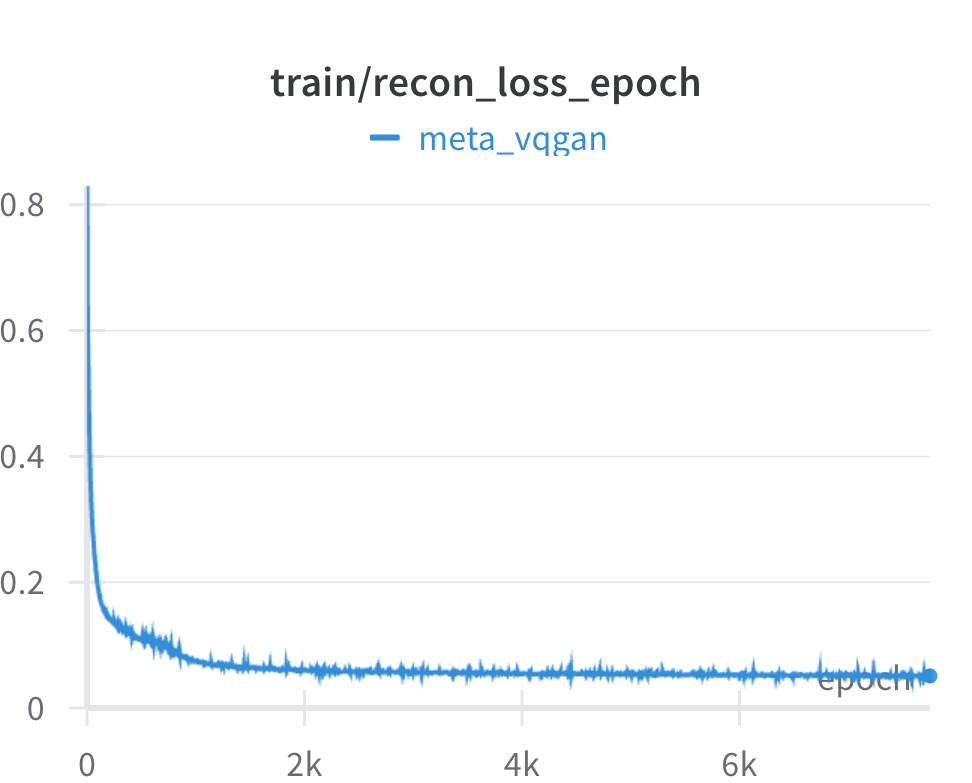
\includegraphics[width=\linewidth]{detailed_engineering/Meta VQGAN/charts/Section-2-Panel-13-1qhe42yar.png}
\caption{Commitment loss during the training.}
\endminipage\hfill
\minipage{0.49\textwidth}
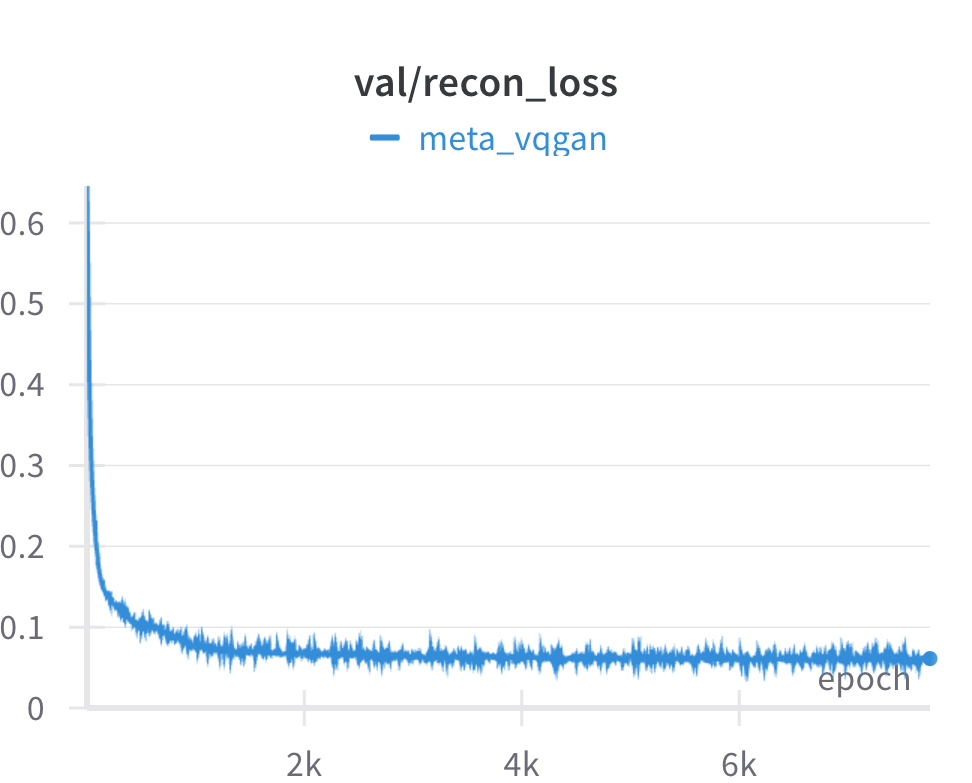
\includegraphics[width=\linewidth]{detailed_engineering/Meta VQGAN/charts/Section-4-Panel-3-hkj1c12xb.png}
\caption{Commitment loss during the validation.}
\endminipage
\caption{Commitment loss during the training and the validation. Lower is better.}
\end{figure}

\begin{figure}[H]
\minipage{0.49\textwidth}
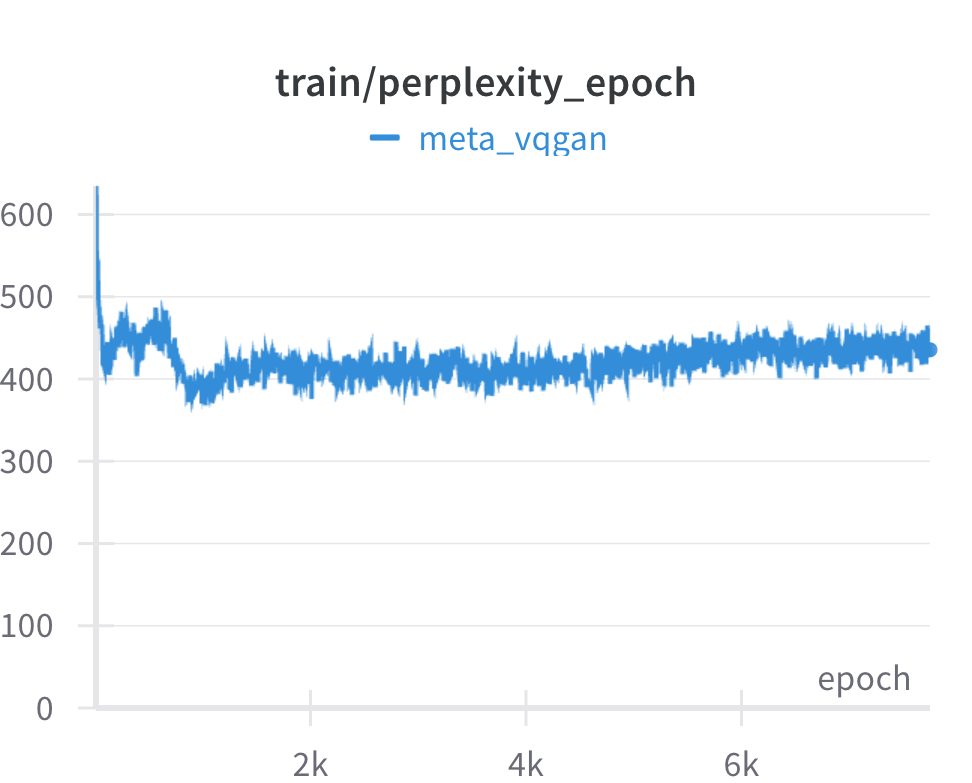
\includegraphics[width=\linewidth]{detailed_engineering/Meta VQGAN/charts/Section-2-Panel-1-5nrgzgmoj.png}
\caption{Perplexity during the training.}
\endminipage\hfill
\minipage{0.49\textwidth}
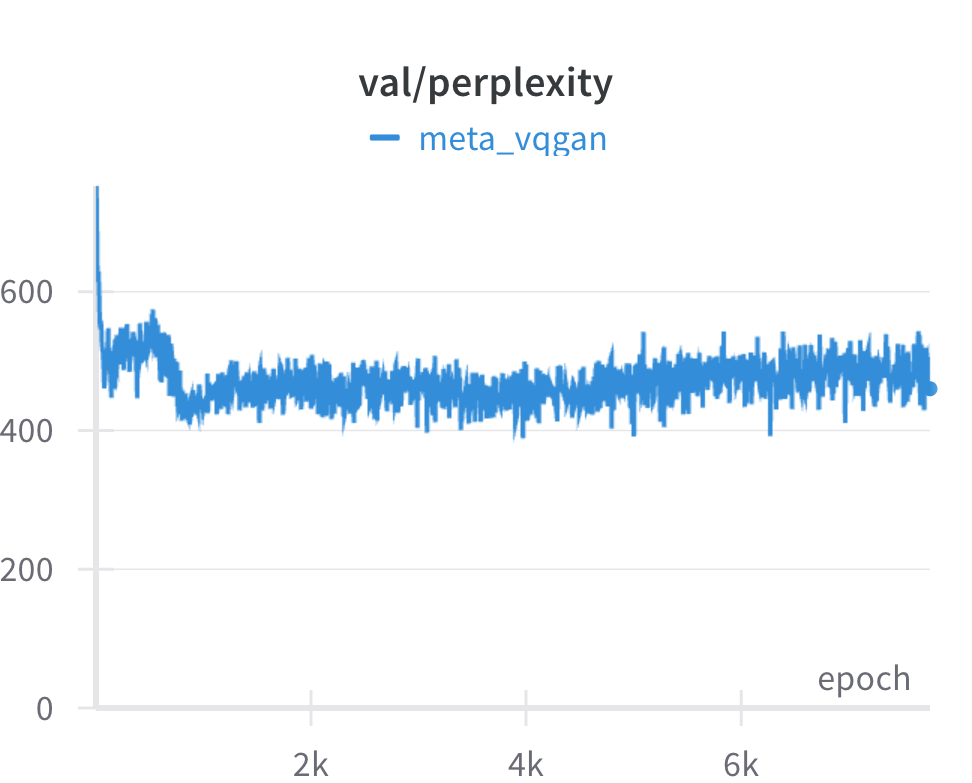
\includegraphics[width=\linewidth]{detailed_engineering/Meta VQGAN/charts/Section-4-Panel-1-njiwngfn7.png}
\caption{Perplexity during the validation.}
\endminipage
\caption{Codebook utilisation during the training and the validation. Higher is better.}
\end{figure}


\paragraph{Evaluation}\mbox{}
\begin{table}[h!]
\centering
\begin{tabular}{|c|c|c|c|c|}
\hline
\textbf{Metric} & VAE & VQVAE1 & Medical Diffusion VQVAE & \textbf{LDM} \\
\hline
$\overline{L1}$ & 0.0309 & 0.0212 & 0.0144 & 0.0845 \\
\hline
$\overline{L2}$ & 0.0043 & 0.0023 & 0.0007 & 0.0270 \\
\hline
$\overline{SSIM}$ & 0.8690 & 0.9399 & 0.9795 & 0.5954 \\
\hline
$\overline{LPIPS}$ & 2.2485 & 1.3820 & 0.8898 & 3.3926 \\
\hline
\end{tabular}
\caption{Mean metrics of the model on the whole dataset as inputs and their reconstructions.}
\label{table:metrics}
\end{table}